\label{capitolo2}
\section{Sistemi di storage}
Le principali richieste che i nuovi sistemi di storage devono soddisfare sono di diversa natura; prima fra tutti la sicurezza dei dati in quanto essi non devono essere corrotti o persi. La reperibilit� dei dati in quanto essi devono essere disponibili 7 giorni su 7 e 24 ore su 24 e disponibili per tutti gli utenti con determinati vincoli. Infine l'espansione dei sistemi di storage deve essere trasparente agli utenti finali.
Queste caratteristiche hanno fatto in modo che i sistemi di storage si evolvessero da \emph{Direct Attached Storage} (DAS) nel quale si aveva una visione centrata sull'host ad una logica di \emph{Storage Area Network} (SAN) centrata sulla rete.\\
Il modello fisico di come sono strutturate le diverse architetture � mostrato in figura \ref{fig:modellofis}
\begin{figure}[ht]
\centering
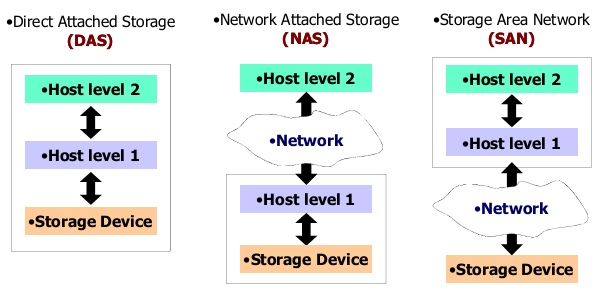
\includegraphics[width=10cm]{img/modellofis.png}
\caption{Modello fisico delle varie architetture di storage}
\label{fig:modellofis}
\end{figure}
Il modello logico � invece rappresentato in figura \ref{fig:modellolog}
\begin{figure}[ht]
\centering
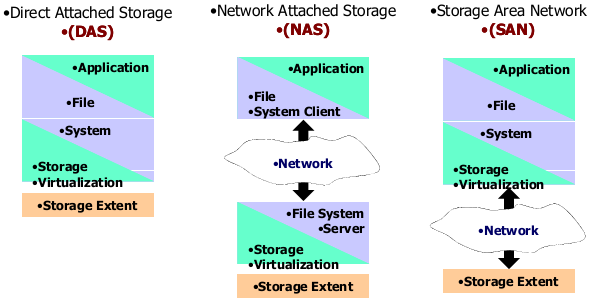
\includegraphics[width=10cm]{img/modellolog.png}
\caption{Modello logico delle varie architetture di storage}
\label{fig:modellolog}
\end{figure}
\subsection{Direct Attached Storage}
Come si nota schema logico di figura \ref{fig:daslog} nei sistemi DAS l'architettura � concentrata su un unica macchina, se si volesse accedere ai dati bisognerebbe passare dalla macchina che ospita il disco. Questo implica i classici problemi di compatibilit� tra i vari sistemi operativi.
\begin{figure}[ht]
\centering
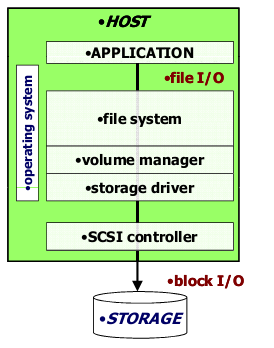
\includegraphics[height=7cm]{img/daslog.png}
\caption{Modello logico dell'architettura DAS}
\label{fig:daslog}
\end{figure}
Questo tipo di architettura rapportata ad un contesto di rete come quello di figura \ref{fig:dasrete} implica grossi problemi di scalabilit� una complessit� molto elevata e prestazioni limitate.
\begin{figure}[ht]
\centering
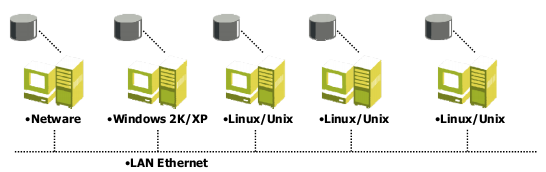
\includegraphics[width=10cm]{img/dasrete.png}
\caption{Modello di rete DAS}
\label{fig:dasrete}
\end{figure}
\subsection{Network Attached Storage}
Il modello logico dell'architettura NAS � rappresentato in figura \ref{fig:naslog}; come si vede questo tipo di architettura prevede un unico sistema che gestisce i dischi questo permette di rendere trasparenti i meccanismi di gestione dei dischi ai diversi host come l'aumento o la sostituzioni di dischi.
\begin{figure}[htb]
\centering
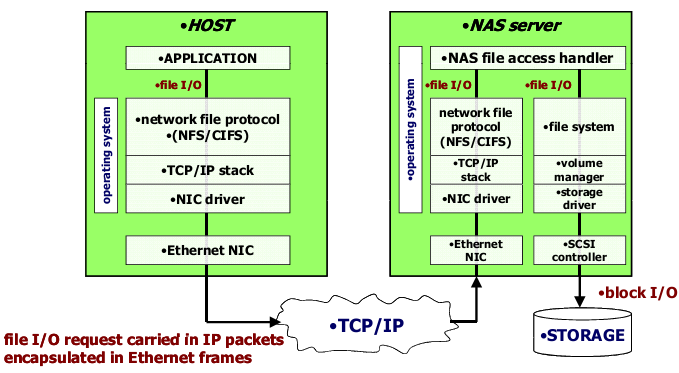
\includegraphics[width=11cm]{img/naslog.png}
\caption{Schema logico dell'architettura NAS}
\label{fig:naslog}
\end{figure}
Il vantaggio principale � la grande scalabilit� basta aggiungere un disco al NAS o una unit� NAS.
Come si vede dallo schema di rete in figura \ref{fig:nasrete} ogni unit� NAS ottiene un indirizzo IP dalla rete.
\begin{figure}[htb]
\centering
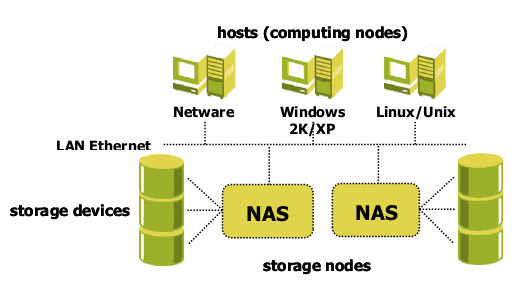
\includegraphics[width=11cm]{img/nasrete.png}
\caption{Schema di rete dell'architettura NAS}
\label{fig:nasrete}
\end{figure}
\subsection{Storage Area Network}
Parliamo di una rete dedicata all'accesso ai dischi. Di solito la comunicazione in questa rete avviene attraverso fibra ottica. Come front-end per gli host si pu� utilizzare un interfaccia NAS in modo da rendere ancora pi� trasparente il sistema di storage come in figura \ref{fig:nassan}
\begin{figure}[hbt]
\centering
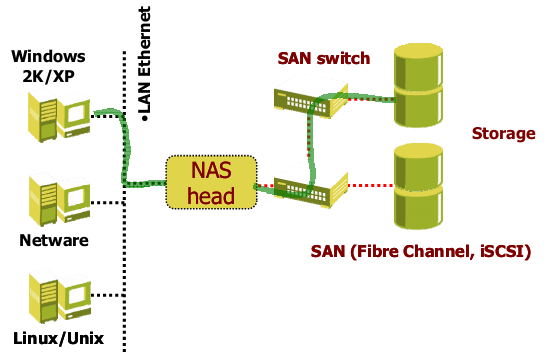
\includegraphics[width=11cm]{img/nassan.png}
\caption{Schema di rete dell'architettura SAN con front-end NAS}
\label{fig:nassan}
\end{figure}
Il vantaggio di questo tipo di rete � la grande scalabilit� in quanto basta aggiungere dei device alla sottorete SAN per aumentare la capacit� dell'intero sistema senza nessun'altra operazione.
\subsubsection*{Fiber Channel}
Solitamente tutta la sottorete SAN � cablata in fibra ottica. In quanto un eventuale cablaggio ethernet implicherebbe numerosi problemi, il primo e pi� importante � quello dell'overhead introdotto dal protocollo TCP/IP a numerosi livelli, per manipolare le trame nella rete o per instradarle attraverso i vari indirizzi ip. Tutte queste informazioni sono inutili in un contesto di storage perci� � preferibile utilizzare un protocollo pi� performante come il \emph{Fiber Channel}.
Il Fiber Channel unisce tutte le caratteristiche migliori per un protocollo mirato allo scambio di grandi quantit� di dati. Alta velocit� nello scambio di dati, alta flessibilit� e la capacit� di realizzare reti estese.
Le caratteristiche principali sono:
\begin{itemize}
\item Collegamenti full-duplex
\item Throughput di 1600 Mbps
\item Supporto per connessioni fino a 10 km
\item Connettori piccoli
\item Uso di componenti standard
\end{itemize}
